\documentclass[10pt]{beamer}

\usepackage[utf8]{inputenc}

\usepackage[T1]{fontenc}

\usepackage{microtype} % microtypographical enhancements

\usepackage[english]{babel}

\usepackage{amsmath, amssymb, amsthm, amsfonts}

\usepackage{graphicx}

\usepackage{bm} % boldface symbols (\bm)

\usepackage{twoopt} % for convenient commands

\usepackage{xfrac} % for \sfrac command

\usepackage{mathrsfs} % calligraphic font \mathscr{C}


\usepackage{dcolumn} % improved alignment of table columns

\usepackage{booktabs} % improved horizontal lines in tables

\usepackage[justification=centering]{caption} % center multiline captions or e.g. [format=hang]



\usepackage[style=alphabetic, backend=biber, isbn=false, url=false, doi=false]{biblatex}

\addbibresource{thesis.bib}


\usepackage{tikz}

\usetikzlibrary{positioning,decorations.markings}
\tikzset{croot/.style={circle,draw,fill=black,inner sep=0pt,minimum size=2mm},
	 nroot/.style={circle,draw,inner sep=0pt,minimum size=2mm},
	 node distance = 1
	 }



\newcommand{\inserttikzfigure}[2]{
											\begin{center}
												\begin{figure}[h]
													\centering 
													\input{#1}
													\caption{#2}
												\end{figure} 
											\end{center}
										}										
%%%%%%%%%%%%%%%%%%%%%%%%%%%%%%%% THEOREMS %%%%%%%%%%%%%%%%%%%%%%%%%%%%%%%%%%

%%%%%%%% CMUC %%%%%%%%%%

%%%%%%%%%%%%%%%%%%%%%%%%%%%%%%%% SYMBOLS %%%%%%%%%%%%%%%%%%%%%%%%%%%%%%%%%%
\newcommand{\et}{\,\&\,}
\renewcommand{\k}{\Bbbk}
\renewcommand{\C}{\mathbb{C}}
\newcommand{\octo}{\mathbb{O}}
\newcommand{\R}{\mathbb{R}}
\newcommand{\N}{\mathbb{N}}
\newcommand{\Z}{\mathbb{Z}}
\newcommand{\lie}[1]{\mathfrak{#1}}
\newcommand{\rep}[1]{\mathbb{#1}}
\newcommand{\bun}[1]{\mathcal{#1}}
\newcommand{\oppar}{\overline{\lie{p}}}
\newcommand{\Hom}{\mathrm{Hom}}
\newcommand{\pproj}[1]{\Pi_{#1}^\lie{g}}
\newcommand{\floor}[1]{\left[ #1 \right]}

\newcommand{\roots}{\Phi} % the set of roots
\newcommand{\sroots}{\Delta} % the set of positive simple roots
\newcommand{\weights}{\Lambda} % weight lattice

\renewcommand{\a}{\alpha}
%%%%%%%%%%%%%%%%%%%%%%%%%%%%%%%% OPERATORS %%%%%%%%%%%%%%%%%%%%%%%%%%%%%%%%%%

%\newcommand{\im}{\mathrm{im}\,}
%\newcommand{\lap}{\square}
%\newcommand{\td}{\mathrm{d}^\lie{g}}
%\newcommand{\id}{\mathrm{Id}\,}
%\newcommand{\plap}{\lap_\lie{g}}
%\newcommand{\lcd}{\partial\,}
% \renewcommand{\lhd}{\mathop{\partial^*}}
% \renewcommand{\lhd}{\mathop{\delta}}
 \renewcommand{\lhd}{\operatorname{\delta}}

\newcommand{\bigo}{\mathcal{O}}

\newcommand{\conj}[1]{\overline{#1}}
\newcommand{\jscal}[2]{\langle #1\,|\, #2 \rangle}
\newcommand{\oscal}[2]{\left( #1 \,|\, #2 \right)}
 

% \DeclareMathOperator{\hom}
\DeclareMathOperator{\proj}{\mathrm{proj}}
\DeclareMathOperator{\im}{\mathrm{im}}
\DeclareMathOperator{\lap}{\square}
\DeclareMathOperator{\id}{\mathrm{Id}}
\DeclareMathOperator{\td}{\mathrm{d}^\lie{g}}
\DeclareMathOperator{\plap}{\lap_\lie{g}}
\DeclareMathOperator{\lcd}{\partial}
% \DeclareMathOperator{\lhd}{\partial^*}
\DeclareMathOperator{\tr}{\mathrm{Tr}}
\DeclareMathOperator{\ad}{\mathrm{ad}}
\DeclareMathOperator{\Ad}{\mathrm{Ad}}
\DeclareMathOperator{\Id}{\mathrm{Id}}

%%%%%%%%%%%%%%%%%%%%%%%%%%%%%%%% ENVIRONMENTS %%%%%%%%%%%%%%%%%%%%%%%%%%%%%%%%%%

\newenvironment{smatrix}{\left(\begin{smallmatrix}}{\end{smallmatrix}\right)}

%%%%%%%%%%%%%%%%%%%%%%%%%% CD %%%%%%%%%%%%%%%%%%%%%%%%%%%%%%%%%%%%%%%%%%%%%%%%%%%%

\newcommand{\dsum}{\oplus}               % small direct sum
\newcommand{\Dsum}{\bigoplus}            % big direct sum
\newcommand{\tens}{\mathbin{\otimes}}    % small tensor product
\newcommand{\Tens}{\bigotimes}           % big tensor product
\newcommand{\cartan}{\mathbin{\odot}}    % small Cartan product
\newcommand{\Cartan}{\bigodot}           % big Cartan product
\newcommand{\subideal}{\ltimes}          % semidirect product for algebras
\newcommand{\idealsub}{\rtimes}          %  with ideal on right or left
\newcommand{\subnormal}{\ltimes}         % semidirect product for groups with
\newcommand{\normalsub}{\rtimes}         %  normal subgroup on right or left
\newcommand{\intersect}{\mathinner{\cap}}% intersection
\newcommand{\setdif}{\mathbin{\mathrm -}}% or {\smallsetminus}
\newcommand{\skwend}{\mathinner{\vartriangle}} % skew endomorphism
%
\newcommand{\act}{\mathinner{\cdot}}
\newcommand{\dual}{^{*\!}}
\newcommand{\Cinf}{\mathrm{C}^\infty}
%
\newcommand{\oper}[3][n]{\newcommand{#2}{\mathop{\mathrm{#3}}\ifx
  n#1\nolimits\else\limits\fi}}
\newcommand{\rsoper}[3][n]{\newcommand{#2}{\mathop{\mathrmsl{#3\mkern1mu}}\ifx
  n#1\nolimits\else\limits\fi}}
\newcommand{\symb}[2]{\newcommand{#1}{{\mathit{#2}}}}
\newcommand{\rssymb}[2]{\newcommand{#1}{{\mathrmsl{#2\mkern1mu}}}}
\newcommand{\calsymb}[2]{\newcommand{#1}{{\mathcal{#2}}}}
\newcommand{\bbsymb}[2]{\newcommand{#1}{{\mathbb{#2}}}}

\rsoper\kernel{ker}
\rsoper\image{im}
% \rsoper\alt{alt}           % alternating part
\rsoper\sym{sym}           % symmetric part
\rsoper\trace{tr}          % trace of an endomorphism
\rsoper\detm{det}          % determinant
\rsoper\divg{div}
\rsoper\Sdivg{Sdiv}
\rsoper\Twist{Twist}
\rsoper\project{proj}
\rsoper\represent{repr}
\rssymb\ev{ev}
\rssymb\iden{id}
%
\newcommand{\cross}{\mathbin{{\times}\!}\low}
\newcommand{\from}{\colon}
\newcommand{\isom}{\cong}
\newcommand{\hQuabla}{\hat{\pmb\square}}
\newcommand{\Quabla}{\pmb{\square}}
\newcommand{\Lie}{{\mathcal L}}
%
\newcommand{\conf}{\mathsf{c}}
\newcommand{\cip}{\ip}
\newcommand{\cform}{\eta}
\newcommand{\g}{\lie{g}}
\newcommand{\p}{\lie{p}}
\newcommand{\Lieb}[1]{[#1]}
\bbsymb\E{E}\bbsymb\W{W}
\newcommand{\T}{\lie{m}}
\newcommand{\inner}{\mathbin{\lrcorner}}
\newcommand{\capinner}{\mathbin{\lower3pt\hbox{$\urcorner$}}}
\newcommand{\low}{^{\vphantom x}}
\newcommand{\dT}{d\low_{\T}}
\newcommand{\dTd}{d\low_{\T^*}}
\newcommand{\delT}{\delta\low_{\T}}
\newcommand{\delTd}{\delta\low_{\T^*}}
\newcommand{\delTdM}{\delta\low_{T\dual M}}
\newcommand{\gM}{\g\low_M}
\newcommand{\InvDer}{\nabla^\cform}
\newcommand{\TwConn}{\nabla^\g}
\newcommand{\deltw}{\delta^\g}
\newcommand{\dtw}{d^\g}
\newcommand{\Rtw}{R^\g}
\newcommand{\QuaTw}{\Quabla_\g}
\newcommand{\Qtw}{Q}
\newcommand{\PiTw}{\Pi}
\calsymb\cD{D}\calsymb\cG{G}\calsymb\cH{H}\calsymb\cK{K}\calsymb\cL{L}

\newcommand{\OpTw}{\cD}
\newcommand{\cptw}{\mathbin{\scriptstyle\sqcup}}
\newcommand{\delinv}{\delta^\cform}
\newcommand{\dinv}{d^\cform}
\newcommand{\Rinv}{R^\cform}
\newcommand{\hQuaInv}{\hQuabla_\cform}
\newcommand{\QuaInv}{\Quabla_\cform}
\newcommand{\Qinv}{Q_\cform}
\newcommand{\PiInv}{\Pi^\cform}
\newcommand{\OpInv}{\cD^\cform}
\newcommand{\Opinv}{\cD_\cform}
\newcommand{\cpinv}{\cptw\low_\cform}
\newcommand{\TwIso}{\Psi_\W}
\newcommand{\captw}{\mathbin{\scriptstyle\sqcap}}
\newcommand{\capinv}{\captw\low_\cform}
\newcommand{\Dirac}{{\smash{\raise1pt\hbox{$\not$}}\mkern-1.5mu D}}

%%%%%%%%%%%%% F4/Spin9
\newcommand{\field}{\Bbbk}
\newcommand{\reals}{\mathbb{R}}
\newcommand{\complex}{\mathbb{C}}
\newcommandtwoopt{\projplane}[2][2][P]{\mathbb{O}{#2}^{#1}}
\newcommandtwoopt{\jalg}[2][G][\octo]{J_{#1}(#2)}

\newcommand{\set}[1]{\left\lbrace #1\right\rbrace}
\renewcommand{\mid}{\middle \mid}
\newcommand{\sform}[1]{\mathrm{II}(#1)}

\newenvironment{psmatrix}
  {\left(\begin{smallmatrix}}
  {\end{smallmatrix}\right)}
	
	%%%%%%%%%%%%%%%%%% G2/P1
	
	\newcommand{\uenv}[1]{\mathfrak{U(#1)}}


\newcommand{\pd}[1]{\partial_{#1}}
\newcommand{\euler}{\mathbb{E}}
\newcommand{\wdeg}{\mathrm{wdeg}\,}
\newcommand{\actpol}{\widehat{\pi}_{\lambda}}

\newcommand{\cas}{\mathrm{Cas}_\mathbb{V}\,}
\newcommand{\vsingtop}{v_\mathrm{sing}^\mathrm{top}}

%%%% 1-graded 

\newcommand{\SL}{\mathrm{SL}}
\def\diag{\mathop {\rm diag} \nolimits}
\let\veps=\varepsilon
%\newcommand*\widebar[1]{\@ifnextchar^{{\wide@bar{#1}{0}}}{\wide@bar{#1}{1}}}
\newcommand{\widebar}[1]{\overline{#1}}
\def\htt{\mathop {\rm ht} \nolimits}
\newcommand{\eus}{\EuScript}
%\let\eus=\EuScript
\let\rarr=\rightarrow
\let\mfrak=\mathfrak
\newcommand{\mcal}{\mathcal}
\def\End{\mathop {\rm End} \nolimits}
\newcommand*\riso{%
  \xrightarrow[]{\raisebox{-0.25em}{\smash{\ensuremath{\sim}}}}%
}
\def\Sol{\mathop {\rm Sol} \nolimits}


\usepackage{threeparttable,array}

\newcolumntype{C}{>{$\displaystyle}c <{$}}


\usetheme[progressbar=frametitle]{metropolis}

\usepackage{appendixnumberbeamer}


\usepackage{booktabs}

\usepackage[scale=2]{ccicons}


\usepackage{pgfplots}

\usepgfplotslibrary{dateplot}


\usepackage{xspace}

\newcommand{\themename}{\textbf{\textsc{metropolis}}\xspace}


\title{Cohomology of unitary representations for Hermitian symmetric spaces}

\subtitle{ECI \et JČMF Workshop -- Telč 2017}

% \date{\today}

\date{}

\author{Vít Tuček}

\institute{Mathematical Institute of Charles University}

\titlegraphic{\hfill
\includegraphics[height=1.7cm]{logo-en.pdf}}


\begin{document}

\metroset{titleformat frame=smallcaps}

\maketitle


\begin{frame}{Table of contents}

\setbeamertemplate{section in toc}[sections numbered]

\tableofcontents[hideallsubsections]

\end{frame}


%\begin{frame}{Animation}

% \begin{itemize}[<+- | alert@+>]

% \item \alert<4>{This is\only<4>{ really} important}

% \item Now this

% \item And now this

% \end{itemize}

%\end{frame}


\section{Hermitian symmetric spaces}


\begin{frame}{Definition -- Hermitian symmetric space}

\begin{itemize}%[<+- | alert@+>]
\item Compact symmetric space $H/K$ is called a Hermitian symmetric space if it admits $H$-invariant complex structure
\item $H/K \simeq G/P$ where $G$ is a complexification of $H$ and $P$ is a parabolic subgroup with \emph{abelian} radical
\item The Levi part of $P$ is complexification of the maximal compact subgroup $K$
%\item The noncompact dual $H^*$ is given on the level of Lie algebras by $\lie{h}^* = \lie{k} \oplus \imath \lie{m}$ where $\lie{h} = \lie{k} \oplus \lie{m}$
%\item Borel embedding $H^*/K \hookrightarrow G/P$
%\item Harish-Chandra embedding $H^*/K \hookrightarrow \lie{m}_+$ where $\lie{m}_+$ is the nilradical of $\lie{p}$
\end{itemize}

\end{frame}


\begin{frame}{Classification}

$
 I_{m,n} = \begin{pmatrix} \Id_m & 0 \\ 0 & -\Id_n \end{pmatrix} \quad J = \begin{pmatrix} 0 & \Id_n \\ -\Id_n & 0 \end{pmatrix} \quad X^\dag = \overline{X}^t
$

\vspace{0.2cm}
\begin{equation*}
\begin{aligned}
\alert{\mathrm{SU}(p,q)} &= \{ g \in \mathrm{GL}(p +q, \mathbb{C}) \,|\, g I_{p,q}g^\dag = I_{p,q} \}\\[0.5cm]
\mathrm{Sp}(n, \mathbb{C}) &= \{ g \in \mathrm{GL}(2n, \mathbb{C}) \,|\, g^t J g  = J \}\\
\alert{\mathrm{Sp}(n, \mathbb{R})} &= \mathrm{Sp}(n, \mathbb{C}) \cap \mathrm{SU}(n,n) \\[0.5cm]
\mathrm{O}(2n, \mathbb{C}) &= \{ g \in \mathrm{GL}(n, \mathbb{C}) \,|\, g^t JI_{n,n} g  = JI_{n,n} \}\\
\alert{\mathrm{SO}^*(2n)} &=  \mathrm{O}(2n, \mathbb{C}) \cap \mathrm{SU}(n,n) \\
\alert{\mathrm{SO}(2, n)} &= \{ g \in \mathrm{GL}(n, \mathbb{R})\,|\, g^t I_{2,n} g  = I_{2,n} \}
\end{aligned}
\end{equation*}

\alert{
\[
	\mathrm{E^{-25}_7 / U(1)E_6^\text{cpt} \quad E^{-14}_6 / U(1)Spin(10)} 
\]
}
\end{frame}

\begin{frame}{Classification}
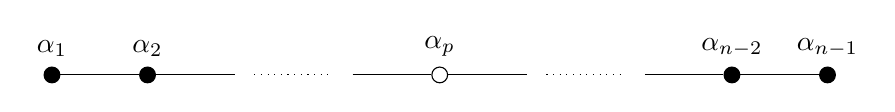
\begin{tikzpicture} % SU(p,q) ~ A_{n-1} relative
	\node[croot] (a1) [label=above:$\alpha_1$] {};
	\node[croot] (a2) [right= of a1] [label=above:$\alpha_2$] {};
	\node (a3) [right= of a2] {};
	\node (a4) [right= of a3] {};
	\node[nroot] (a5) [right=of a4] [label=above:$\alpha_p$] {};
	\node (a6) [right= of a5] {};
	\node (a7) [right=of a6] {};
	\node[croot] (a8) [right=of a7] [label=above:$\alpha_{n-2}$] {};
	\node[croot] (a9) [right=of a8] [label=above:$\alpha_{n-1}$] {};
	\draw (a1) to (a2) to (a3); \draw [dotted] (a3) to (a4);
	\draw (a4) to (a5) to (a6); \draw [dotted](a6) to (a7);
	\draw (a7) to (a8) to (a9);
\end{tikzpicture}

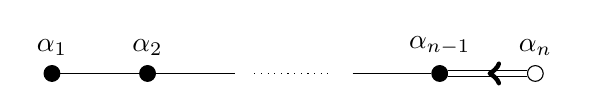
\begin{tikzpicture}[decoration={markings,mark=at position .5 with {\arrowreversed[line width=2pt]{>}}}] % Sp(n,\R) ~ C_n relative
	\node[croot] (a1) [label=above:$\alpha_1$] {};
	\node[croot] (a2) [right= of a1] [label=above:$\alpha_2$] {};
	\node (a3) [right= of a2] {};
	\node (a4) [right= of a3] {};
	\node[croot] (a5) [right=of a4] [label=above:$\alpha_{n-1}$] {};
	\node[nroot] (a6) [right=of a5] [label=above:$\alpha_{n}$] {};
	\draw (a1) to (a2) to (a3); \draw [dotted] (a3) to (a4);
	\draw (a4) to (a5); \draw [postaction={decorate},double distance=1.5pt] (a5) to (a6);
\end{tikzpicture}	
\begin{tikzpicture} % SO^*(2n) ~ D_n relative
	\node[croot] (a1) [label=above:$\alpha_1$] {};
	\node[croot] (a2) [right= of a1] [label=above:$\alpha_2$] {};
	\node (a3) [right= of a2] {};
	\node (a4) [right= of a3] {};
	\node[croot] (a5) [right= of a4] [label=above left:$\alpha_{n-2}$] {};
	\node[nroot] (a6) [above right= of a5] [label=above:$\alpha_{n}$] {};
	\node[croot] (a7) [below right= of a5] [label=above right:$\alpha_{n-1}$] {};
	\draw (a1) to (a2) to (a3);
	\draw [dotted] (a3) to (a4);
	\draw (a4) to (a5) to (a6);
	\draw (a5) to (a7);
\end{tikzpicture}
	
\begin{tikzpicture} % SO^*(2n) ~ D_n relative
	\node[nroot] (a1) [label=above:$\alpha_1$] {};
	\node[croot] (a2) [right= of a1] [label=above:$\alpha_2$] {};
	\node (a3) [right= of a2] {};
	\node (a4) [right= of a3] {};
	\node[croot] (a5) [right= of a4] [label=above left:$\alpha_{n-2}$] {};
	\node[croot] (a6) [above right= of a5] [label=above:$\alpha_{n}$] {};
	\node[croot] (a7) [below right= of a5] [label=above right:$\alpha_{n-1}$] {};
	\draw (a1) to (a2) to (a3);
	\draw [dotted] (a3) to (a4);
	\draw (a4) to (a5) to (a6);
	\draw (a5) to (a7);
\end{tikzpicture}	
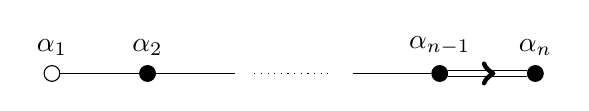
\begin{tikzpicture}[decoration={markings,mark=at position .6 with {\arrow[line width=2pt]{>}}}] % SO(2n-1,\R) ~ B_n relative
	\node[nroot] (a1) [label=above:$\alpha_1$] {};
	\node[croot] (a2) [right= of a1] [label=above:$\alpha_2$] {};
	\node (a3) [right= of a2] {};
	\node (a4) [right= of a3] {};
	\node[croot] (a5) [right=of a4] [label=above:$\alpha_{n-1}$] {};
	\node[croot] (a6) [right=of a5] [label=above:$\alpha_{n}$] {};
	\draw (a1) to (a2) to (a3); \draw [dotted] (a3) to (a4);
	\draw (a4) to (a5); \draw [postaction={decorate},double distance=1.5pt] (a5) to (a6);
\end{tikzpicture}

\end{frame}

\begin{frame}{Classification}
    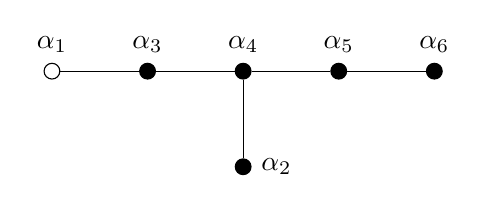
\begin{tikzpicture}% E6 relative
        \node[nroot] (a1) [label=above:$\alpha_1$] {};
        \node[croot] (a3) [right=of a1] [label=above:$\alpha_3$] {};
        \node[croot] (a4) [right=of a3] [label=above:$\alpha_4$] {};
        \node[croot] (a5) [right=of a4] [label=above:$\alpha_5$] {};
        \node[croot] (a6) [right=of a5] [label=above:$\alpha_6$] {};
        \node[croot] (a2) [below=of a4] [label=right:$\alpha_2$] {};
        \draw (a1) to (a3) to (a4) to (a5) to (a6);
        \draw (a4) to (a2);
     \end{tikzpicture}
		
		     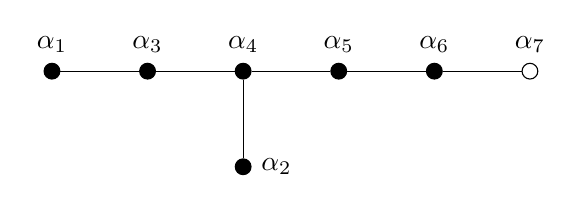
\begin{tikzpicture} % E7 relative
        \node[croot] (a1) [label=above:$\alpha_1$] {};
        \node[croot] (a3) [right=of a1] [label=above:$\alpha_3$] {};
        \node[croot] (a4) [right=of a3] [label=above:$\alpha_4$] {};
        \node[croot] (a5) [right=of a4] [label=above:$\alpha_5$] {};
        \node[croot] (a6) [right=of a5] [label=above:$\alpha_6$] {};
        \node[nroot] (a7) [right=of a6] [label=above:$\alpha_7$] {};
        \node[croot] (a2) [below=of a4] [label=right:$\alpha_2$] {};
        \draw (a1) to (a3) to (a4) to (a5) to (a6) to (a7);
        \draw (a4) to (a2);
     \end{tikzpicture}
\end{frame}


\begin{frame}{Invariant differential operators}
\begin{itemize}[<+- | alert@+>]
	\item For a homogeneous space $G/H$, $H$-representation $\mathbb{V}$ the associated homogeneous bundle is $\mathcal{V} = G \times_H \mathbb{V} \to G/H$
	\item \emph{invariant differential operators} between sections of two such bundles $\mathcal{V}$ and $\mathcal{W}$ must respect natural induced actions of $G$
	\begin{gather*}
\mathcal{D} \colon \Gamma^\infty(G/H, \mathcal{V}) \to \Gamma^\infty(G/H, \mathcal{W}) \\
\mathcal{D} \circ \widetilde{\rho_\mathbb{V}} =  \widetilde{\rho_\mathbb{W}} \circ \mathcal{D}.
\end{gather*}
\item (linear) differential operator $\mathcal{D}$ of order $k$ is given by a linear map from the $k$-th jet prolongation 
\[
D\colon \Gamma^\infty(G/H,\mathcal{J}^k \mathcal{V}) \to \Gamma^\infty(G/H, \mathcal{W})
\]
\item From invariance we equivalently have homomorphism $J^k \mathbb{V} \to \mathbb{W},$ where  $J^k \mathbb{V}$ denotes the algebraic jet prolongation of $\mathbb{V}.$
\item Passing to dual maps and taking the limit $k \to \infty$ we get 
\[
\Hom_{\mathfrak{h}}\left(\mathbb{W}^*, \, \mathfrak{U(g)\otimes_{U(h)}}\mathbb{V}^*\right) \simeq \Hom_{\mathfrak{g}}\left(\mathfrak{U(g)\otimes_{U(h)}}\mathbb{W}^*, \, \mathfrak{U(g)\otimes_{U(h)}}\mathbb{V}^*\right)
\]
\end{itemize}
 

\end{frame}


\begin{frame}{Invariant differential operators}
\begin{itemize}
	\item Classification in the homogeneous case $G/P$
	\item Natural extension to Cartan geometries modelled on $(G, P)$
\end{itemize}
\end{frame}

%\begin{frame}{Calderbank--Diemer construction}
%\begin{itemize}[<+- | alert@+>]
	%\item Certain Neumann series has to converge $\rightsquigarrow$ formal globalization
	%\item formal globalization has a well defined $P$-action\\ \hspace{1cm} $\rightsquigarrow$ highest / lowest weight
	%\item operator in the Neumann series constructed using Kostant's Hodge decomposition $\rightsquigarrow$ unitarizable modules
%\end{itemize}
%\end{frame}


\section{Unitarizable highest weight modules}
%

\begin{frame}{Classification}
\begin{itemize}[<+- | alert@+>]
	\item Exists only for the Hermitian symmetric pairs. 
	\item Given by the simple quotient $L(\lambda)$ of a parabolic Verma module $M(\lambda) = \mathfrak{U(g)\otimes_{U(p)}}\mathbb{F}_\lambda$
	\item Hermitian product given by the \emph{Shapovalov form}
\end{itemize}
\end{frame}

\begin{frame}{Classification --- continued}
\begin{itemize}[<+- | alert@+>]
\item fixing the center of $\lie{k}$ by  $\frac{2 \langle \zeta,\beta \rangle}{\langle \beta, \beta \rangle} = 1$ we can write any weight $\lambda$ uniquely as $\lambda = \lambda_0 + z \zeta$ with  $\langle \lambda_0 + \rho,\beta \rangle = 0$
	\item the set of $z \in \mathbb{C}$ for which the simple factor of Verma module $L(\lambda)$ is unitarizable:
	
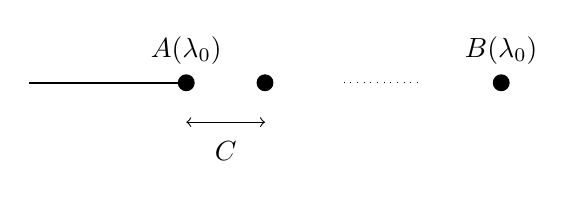
\begin{tikzpicture}
      \node[croot] at (2,0) [label=above:$A(\lambda_0)$] {};
      \node[croot] at (3,0) {};
      \node[croot] at (6,0) [label=above:$B(\lambda_0)$] {};
      \draw[thick] (0,0) to (2,0);
      \draw [dotted] (4,0) to (5,0);
      \draw[<->] (2,-0.5) -- (3,-0.5);
      \node at (2.5,-0.5) [label=below:$C$] {};
  \end{tikzpicture}
	
	$A(\lambda_0)$, $B(\lambda_0)$ and $C(\lambda_0)$ are real numbers expressible in terms of certain root systems $Q(\lambda_0)$ and $R(\lambda_0)$ associated to $\lambda_0$
	
	
\begin{table}[h]
\[\begin{array}{c|ccccccc}
\lie{g} & \mathrm{SU}(p,q) & \mathrm{Sp}(n,\mathbb{R}) & \mathrm{SO}^*(2n) & \mathrm{SO}(2,2n-2) & \mathrm{SO}(2,2n-1) & \mathrm{E}_6 & \mathrm{E}_7\\\hline
C & 1 & \frac{1}{2} & 2 & n-2 & n-\frac{3}{2} & 3 & 4
\end{array}\]\caption{Distance between points of reducibility}\label{tbl:C}
\end{table}
\end{itemize}
\end{frame}

\begin{frame}
$\beta$ \ldots maximal non-compact root
	    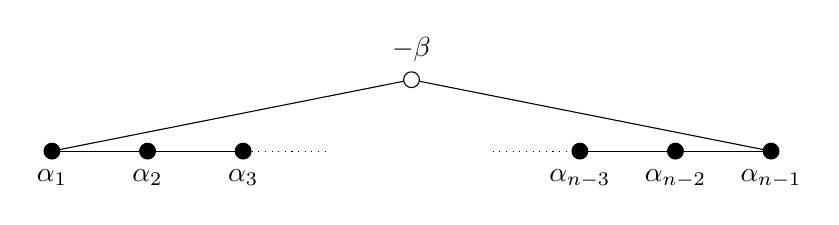
\begin{tikzpicture} % SU(p,q) ~ A_{n-1} relative
	\node[croot] (a1) [label=below:$\alpha_1$] {};
	\node[croot] (a2) [right= of a1] [label=below:$\alpha_2$] {};
	\node[croot] (a3) [right= of a2] [label=below:$\alpha_3$] {};
	\node (a4) [right= of a3] {};
	\node[nroot] (a5) [above right=of a4] [label=above:$-\beta$] {};
	\node (a6) [below right=of a5] {};
	\node[croot] (a7) [right=of a6] [label=below:$\alpha_{n-3}$] {};
	\node[croot] (a8) [right=of a7] [label=below:$\alpha_{n-2}$] {};
	\node[croot] (a9) [right=of a8] [label=below:$\alpha_{n-1}$] {};
	\draw (a1) to (a2) to (a3); \draw [dotted] (a3) to (a4);
	\draw [dotted](a6) to (a7);
	\draw (a7) to (a8) to (a9);
	\draw (a1) to (a5) to (a9);
     \end{tikzpicture}

$Q(\lambda_0)$ \ldots maximal connected subdiagram containing $-\beta$ such that its every compact simple root is orthogonal to $\lambda_0$.
\begin{theorem}[Theorem 2.8 of \cite{enright_classification_1983}]
 Let $\roots^+_{c,1} := \roots^+_c \cap Q(\lambda_0)$ and let $\roots^+_{c,2} := \roots^+_c \cap R(\lambda_0)$. Denote by $\rho_{c,i}$ half of the sum of roots in $\roots^+_{c,i}$.
 
 If $\lie{g}_0=\lie{so}(2,2n-1)$ and $Q(\lambda_0) \neq R(\lambda_0)$ then \[B(\lambda_0) = 1 + \frac{\langle \rho_{c,2},\beta\rangle}{\langle \beta, \beta \rangle}.\]
 In all other cases \[B(\lambda_0) = 1 + \frac{ \langle \rho_{c,1} + \rho_{c,2} , \beta \rangle}{\langle \beta, \beta \rangle}.\]
\end{theorem}

\begin{theorem}[Theorem 2.10 of \cite{enright_classification_1983}]\label{thm:reduction_points}
 The first reduction point $A(\lambda_0)$ is given by\footnote{Or in other words, the number of reduction points equals the split rank of $Q(\lambda_0)$.}
 \[
   A(\lambda_0) = B(\lambda_0) - (\text{split rank of } Q(\lambda_0) -1) C.
 \]
\end{theorem}

\end{frame}


\begin{frame}{Classification -- cone decomposition}

\emph{level of reduction} \ldots \\
$L(\lambda) = M(\lambda) / N(\lambda)$ where $N(\lambda) \subseteq M(\lambda)^k$ for $k\geq l$.

For $\lambda=(B - nC)\zeta + \lambda_0 \in \Lambda_r$ we have $l(\lambda) =n+1$

$a=(Q(\lambda_0), R(\lambda_0), l(\lambda_0))$ for ``reducible'' unitarizable highest weight module

$C_a$  -- integral cone of $\lie{k}$-dominant integral elements in $\lie{h}^*_\R$ which are orthogonal to elements in $R$

The set of reduction points $\Lambda_r$ is the disjoint union of translated integral cones $\lambda_a + C_a$.

\begin{lemma}[Section 4.3 of \cite{enright_resolutions_2004}]
The cone $C_{Q, R, l}$ consists of positive integral multiples of weights of the form $\omega_i - (\omega_i, \beta^\vee) \zeta,$ where $\omega_i$ is a fundamental weight corresponding to simple root $\alpha_i$ that does not belong to $R$.
\end{lemma}
\end{frame}
%

\begin{frame}{Enright's formula}

\begin{definition}\label{def:cohomology_roots}
Let $\Psi_\lambda$ be the set of roots orthogonal to $\lambda+\rho$.

\pause

 Denote by $\roots_{n,\lambda}^+$ the roots which satisfy the following conditions
 \begin{enumerate}
    \item $\alpha \in \roots_n^+$ and $(\lambda+\rho,\alpha^\vee)$ is a positive integer;
    \item $\alpha$ is orthogonal to $\Psi_\lambda$;
    \item $\alpha$ is short if there exist a long root in $\Psi_\lambda$.
 \end{enumerate}

\pause 

 Let $W_\lambda$ be the subgroup of $W$ which is generated by reflections $s_\alpha$ for $\alpha\in \roots_{n,\lambda}^+$.

\pause 

 Let $\roots_\lambda$ be the subset of $\roots$ of elements $\beta$ with $s_\beta\in W_\lambda$ and let $\roots_{\lambda,c} = \roots_c \cap \roots_\lambda$, $\roots_{\lambda,c}^+ = \roots_{\lambda,c} \cap \roots^+$.

\pause 

 Finally, define  $W^{c,i}_\lambda = \{ w \in W_\lambda \, |\, w \rho \text{ is } \roots^+_{\lambda, c}\text{-dominant and } l_\lambda(w)=i \}$.
\end{definition}

\end{frame}

\begin{frame}{Enright's formula -- continued}
\begin{theorem}[Theorem 3.7 of \cite{davidson_differential_1991}]
 For unitarizable highest weight modules $L(\lambda)$ and for $i\in \mathbb{N}$ we have
\begin{equation*}
 H^i(\lie{p}_+, L(\lambda))\simeq \bigoplus_{w\in W^{c,i}_\lambda} F(\overline{w(\lambda+\rho)} - \rho)
\end{equation*}
where  $\overline{\lambda}$ is the unique $\roots_c^+$-dominant element in the $W_c$ orbit of $\lambda$.
\end{theorem}

\end{frame}


\begin{frame}{Example -- nilpotent cohomology for $ \lie{so}(2,2n-2)$}

$\lie{g} = \lie{so}(2,2n-2)$ with $\lambda = (2-n)\omega_1$

$\lambda + \rho = (1,n-2,\ldots,1,0)$

 $\Psi_\lambda^+ = \{ \epsilon_1 - \epsilon_{n-1}\}$

The only noncompact root that is orthogonal to $\epsilon_1 -  \epsilon_{n-1}$ and whose scalar product with $\lambda + \rho$ is positive integral is $\alpha = \epsilon_1 + \epsilon_{n-1}$. 

Thus we get $\roots_{n,\lambda}^+ = \epsilon_1 + \epsilon_{n-1} = \roots_\lambda$. It follows that
\begin{align*}
 H^0(\lie{p}_-,L((2-n)\omega_1)) &= F((2-n)\omega_1)\\
 H^1(\lie{p}_-,L((2-n)\omega_1)) &= F(-n\omega_1)\\
 H^i(\lie{p}_-,L((2-n)\omega_1)) &= 0 \text{ for } i\geq 2.
\end{align*} 
\end{frame}

\begin{frame}{Example -- nilpotent cohomology for $ \lie{so}(2,2n-1)$}
Similarly for $\lie{g} = \lie{so}(2,2n-1)$ and $\lambda = (3/2 - n)\omega_1$ and we get that in that case
\begin{align*}
 H^0(\lie{p}_-,L((3/2-n)\omega_1)) &= F((3/2-n)\omega_1)\\
 H^1(\lie{p}_-,L((3/2-n)\omega_1)) &= F((-1/2-n)\omega_1)\\
 H^i(\lie{p}_-,L((3/2-n)\omega_1)) &= 0 \text{ for } i\geq 2.
\end{align*}
\end{frame}
%

\begin{frame}{$\mathrm{SO}(2,2n-2), n\geq 3$}
\begin{center}\begin{threeparttable}
\begin{tabular}{CCCCC}
  \text{Vertex } \lambda_a & \text{Weight } \mu_a &  Q(\lambda_a) = R(\lambda_a)& l(\lambda_a) \\ \hline
  -(2n-p-1)\omega_1+\omega_{p+1} & -(2n-p)\omega_1 + \omega_p  & \mathrm{SU}(1,p)\tnote{1} &  1 \\
  -(n+1)\omega_1 +\omega_{n-1} + \omega_n & -(n+2)\omega_1 + \omega_{n-2} & \mathrm{SU}(1,n-2) &  1 \\
  -(n-1)\omega_1 + \omega_n \tnote{2} & -n\omega_1+\omega_{n-1} &  \mathrm{SU}(1,n-1) & 1 \\
  -(n-2)\omega_1 & -n\omega_1 & \mathrm{SO}(2,2n-2) &  2\\
  0 & -2\omega_1 + \omega_2 & \mathrm{SO}(2,2n-2) &  1 \\
  -(n-1)\omega_1  + \omega_{n-1} \tnote{3} & -n\omega_1 + \omega_n &\mathrm{SU}(1,n-1) & 1
\end{tabular}\smallskip
\begin{tablenotes}
 \item [1] $1\leq p \leq n-3$ with Dynkin diagram of $R(\lambda_a)$:\\
 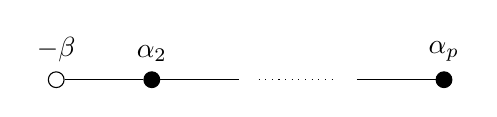
\begin{tikzpicture} % SO^*(2n) ~ D_n relative
	\node[nroot] (a1) [label=above:$-\beta$] {};
	\node[croot] (a2) [right= of a1] [label=above:$\alpha_2$] {};
	\node (a3) [right= of a2] {};
	\node (a4) [right= of a3] {};
	\node[croot] (a5) [right= of a4] [label=above:$\alpha_{p}$] {};
	\draw (a1) to (a2) to (a3);
	\draw [dotted] (a3) to (a4);
	\draw (a4) to (a5);
     \end{tikzpicture}
 \item [2] Dynkin diagram  of $R(\lambda_a)$:
 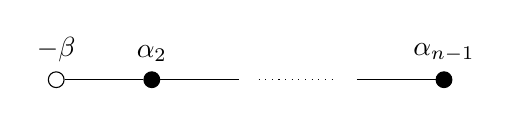
\begin{tikzpicture} % SO^*(2n) ~ D_n relative
	\node[nroot] (a1) [label=above:$-\beta$] {};
	\node[croot] (a2) [right= of a1] [label=above:$\alpha_2$] {};
	\node (a3) [right= of a2] {};
	\node (a4) [right= of a3] {};
	\node[croot] (a5) [right= of a4] [label=above:$\alpha_{n-1}$] {};
	\draw (a1) to (a2) to (a3);
	\draw [dotted] (a3) to (a4);
	\draw (a4) to (a5);
     \end{tikzpicture}
 \item [3] Dynkin diagram of $R(\lambda_a)$:
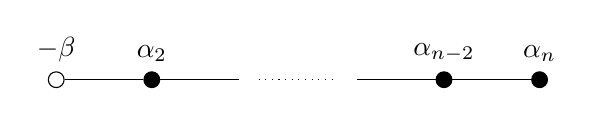
\begin{tikzpicture} % SO^*(2n) ~ D_n relative
	\node[nroot] (a1) [label=above:$-\beta$] {};
	\node[croot] (a2) [right= of a1] [label=above:$\alpha_2$] {};
	\node (a3) [right= of a2] {};
	\node (a4) [right= of a3] {};
	\node[croot] (a5) [right= of a4] [label=above:$\alpha_{n-2}$] {};
	\node[croot] (a6) [right= of a5] [label=above:$\alpha_{n}$] {};
	\draw (a1) to (a2) to (a3);
	\draw [dotted] (a3) to (a4);
	\draw (a4) to (a5) to (a6);
     \end{tikzpicture} 
\end{tablenotes}
\caption{Vertices and root systems for $\mathrm{SO}(2,2n-2)$, $n\geq 3$}\label{tbl:so_even}
\end{threeparttable}\end{center}
\end{frame}

\begin{frame}{$\lambda =  -(2n-p-1)\omega_1+\omega_{p+1}$}
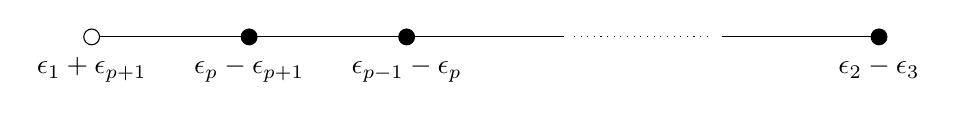
\begin{tikzpicture}
\draw (0 cm,0) -- (6 cm,0);
\draw (8 cm,0) -- (10 cm,0);
\draw[fill=white] (0 cm, 0 cm) circle (.1cm) node[below=4pt]{$\epsilon_{1} + \epsilon_{p+1}$};
\draw[fill=black] (2 cm, 0 cm) circle (.1cm) node[below=4pt]{$\epsilon_{p} - \epsilon_{p+1}$};
\draw[fill=black] (4 cm, 0 cm) circle (.1cm) node[below=4pt]{$\epsilon_{p-1} - \epsilon_{p}$};
\node (node_a) at (6 cm, 0 cm) {};
\node (node_b) at (8 cm, 0 cm) {};
\draw[fill=black] (10 cm, 0 cm) circle (.1cm) node[below=4pt]{$\epsilon_{2} - \epsilon_{3}$};
\draw [dotted] (node_a) to (node_b);
\end{tikzpicture}  
	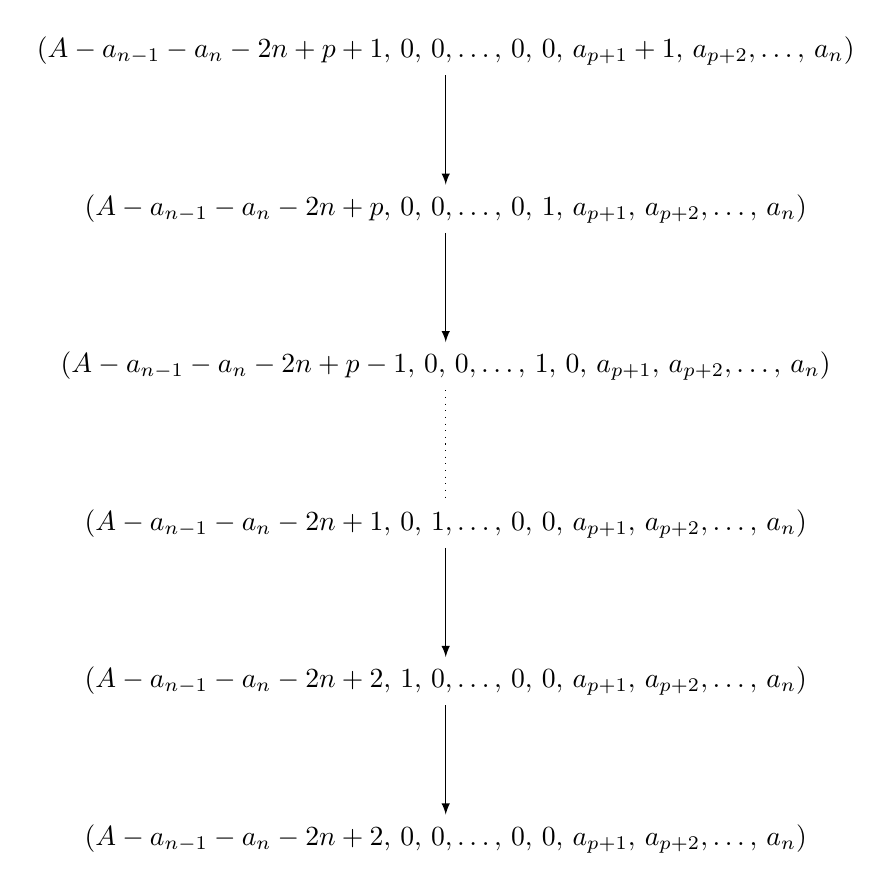
\begin{tikzpicture}[>=latex,line join=bevel,]

  \node (node_0) at (0,10) [draw,draw=none] {$\left(A - a_{n-1} - a_{n} - 2n + p + 1,\,0,\,0,\ldots,\,0,\,0,\,a_{p+1}+1,\,a_{p+2},\ldots,\,a_{n}\right)$};

  \node (node_1) at (0,8) [draw,draw=none] {$\left(A - a_{n-1} - a_{n} - 2n + p,\,0,\,0,\ldots,\,0,\,1,\,a_{p+1},\,a_{p+2},\ldots,\,a_{n}\right)$};

  \node (node_2) at (0,6) [draw,draw=none] {$\left(A - a_{n-1} - a_{n} - 2n + p-1,\,0,\,0,\ldots,\,1,\,0,\,a_{p+1},\,a_{p+2},\ldots,\,a_{n}\right)$};

  \node (node_3) at (0,4) [draw,draw=none] {$\left(A - a_{n-1} - a_{n} - 2n + 1,\,0,\,1,\ldots,\,0,\,0,\,a_{p+1},\,a_{p+2},\ldots,\,a_{n}\right)$};

  \node (node_4) at (0,2) [draw,draw=none] {$\left(A - a_{n-1} - a_{n} - 2n + 2,\,1,\,0,\ldots,\,0,\,0,\,a_{p+1},\,a_{p+2},\ldots,\,a_{n}\right)$};
  
  \node (node_5) at (0,0) [draw,draw=none] {$\left(A - a_{n-1} - a_{n} - 2n +2,\,0,\,0,\ldots,\,0,\,0,\,a_{p+1},\,a_{p+2},\ldots,\,a_{n}\right)$};

  \draw [black,->] (node_0) edge (node_1);
  \draw [black,->] (node_1) edge (node_2);
  \draw [dotted] (node_2) to (node_3);
  \draw [black,->] (node_3) edge (node_4);
  \draw [black,->] (node_4) edge (node_5);
%
\end{tikzpicture}
  Nilpotent cohomology / BGG resolution, $A = -2(a_{p+1} + \cdots + a_{n-2})$
\end{frame}

\begin{frame}{$\lambda = -(a+b+n+1)\omega_1 + (a+1)\omega_{n-1} + (b+1)\omega_n$}
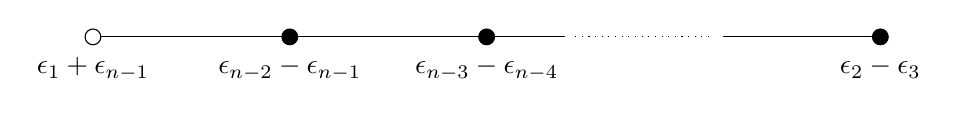
\begin{tikzpicture}
\draw (0 cm,0) -- (6 cm,0);
\draw (8 cm,0) -- (10 cm,0);
\draw[fill=white] (0 cm, 0 cm) circle (.1cm) node[below=4pt]{$\epsilon_{1} + \epsilon_{n-1}$};
\draw[fill=black] (2.5 cm, 0 cm) circle (.1cm) node[below=4pt]{$\epsilon_{n-2} - \epsilon_{n-1}$};
\draw[fill=black] (5 cm, 0 cm) circle (.1cm) node[below=4pt]{$\epsilon_{n-3} - \epsilon_{n-4}$};
\node (node_a) at (6 cm, 0 cm) {};
\node (node_b) at (8 cm, 0 cm) {};
\draw[fill=black] (10 cm, 0 cm) circle (.1cm) node[below=4pt]{$\epsilon_{2} - \epsilon_{3}$};
\draw [dotted] (node_a) to (node_b);
\end{tikzpicture}  
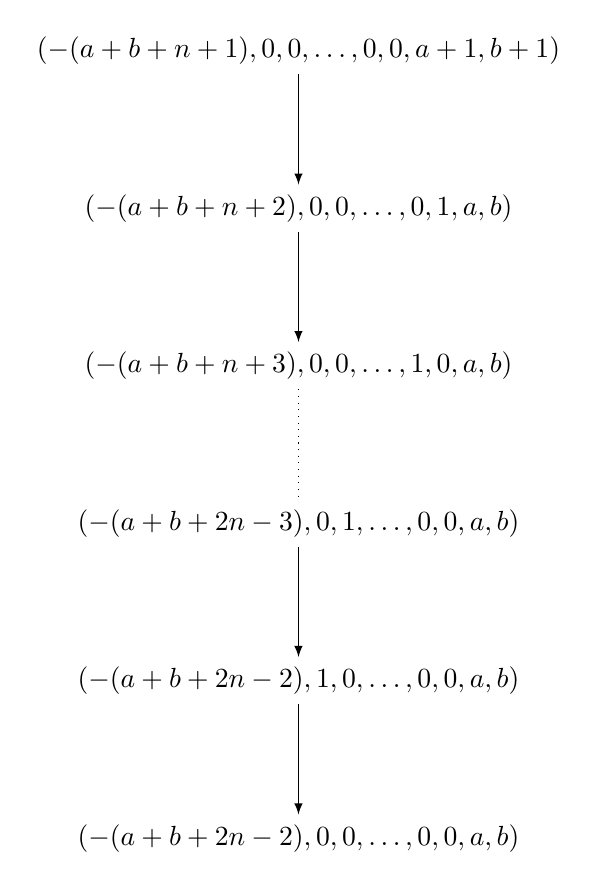
\begin{tikzpicture}[>=latex,line join=bevel,]

  \node (node_0) at (0,10) [draw,draw=none] {$\left(-(a+b+n+1), 0, 0, \ldots, 0, 0, a+1, b+1 \right)$};

  \node (node_1) at (0,8) [draw,draw=none] {$\left(-(a+b+n+2), 0, 0, \ldots, 0, 1, a, b \right)$};

  \node (node_2) at (0,6) [draw,draw=none] {$\left(-(a+b+n+3), 0, 0, \ldots, 1, 0, a, b \right)$};

  \node (node_3) at (0,4) [draw,draw=none] {$\left(-(a+b+2n-3), 0, 1, \ldots, 0, 0, a, b \right)$};

  \node (node_4) at (0,2) [draw,draw=none] {$\left(-(a+b+2n-2), 1, 0, \ldots, 0, 0, a, b \right)$};
  
  \node (node_5) at (0,0) [draw,draw=none] {$\left(-(a+b+2n-2), 0, 0, \ldots, 0, 0, a, b \right)$};

  \draw [black,->] (node_0) edge (node_1);
  \draw [black,->] (node_1) edge (node_2);
  \draw [dotted] (node_2) to (node_3);
  \draw [black,->] (node_3) edge (node_4);
  \draw [black,->] (node_4) edge (node_5);
%
\end{tikzpicture}
	
\end{frame}

\begin{frame}{$\lambda = -(t+n-1)\omega_1 + (t+1)\omega_n$}
For $t=0$ we obtain set of singular roots $\Psi^+_\lambda = \{ \epsilon_1-\epsilon_n\}$ and set generating roots $\roots^+_{n,\lambda} = \{ \epsilon_1 + \epsilon_n \}$. This gives the subsystem of type $A_1$
  \[
   \roots_\lambda = \{ \epsilon_1 + \epsilon_n, -\epsilon_1 - \epsilon_n\}
  \]
  and the resulting weights for nontrivial cohomology groups are all in the table \ref{tbl:so_even}. 
  
  For $t\geq 1$ we get no singular roots $\Psi^+_\lambda = \emptyset$ and the generated subsystem is of type $A_{n-1}.$
	
	
	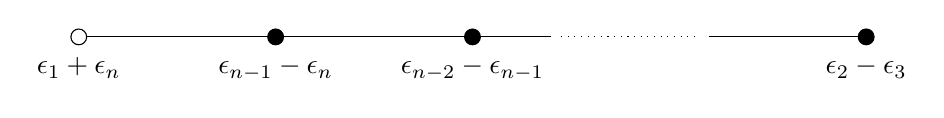
\begin{tikzpicture}
\draw (0 cm,0) -- (6 cm,0);
\draw (8 cm,0) -- (10 cm,0);
\draw[fill=white] (0 cm, 0 cm) circle (.1cm) node[below=4pt]{$\epsilon_{1} + \epsilon_{n}$};
\draw[fill=black] (2.5 cm, 0 cm) circle (.1cm) node[below=4pt]{$\epsilon_{n-1} - \epsilon_{n}$};
\draw[fill=black] (5 cm, 0 cm) circle (.1cm) node[below=4pt]{$\epsilon_{n-2} - \epsilon_{n-1}$};
\node (node_a) at (6 cm, 0 cm) {};
\node (node_b) at (8 cm, 0 cm) {};
\draw[fill=black] (10 cm, 0 cm) circle (.1cm) node[below=4pt]{$\epsilon_{2} - \epsilon_{3}$};
\draw [dotted] (node_a) to (node_b);
\end{tikzpicture}  
  {The reduced Hermitian symmetric pair for $\lambda = -(n-1)\omega_1 + \omega_n$}


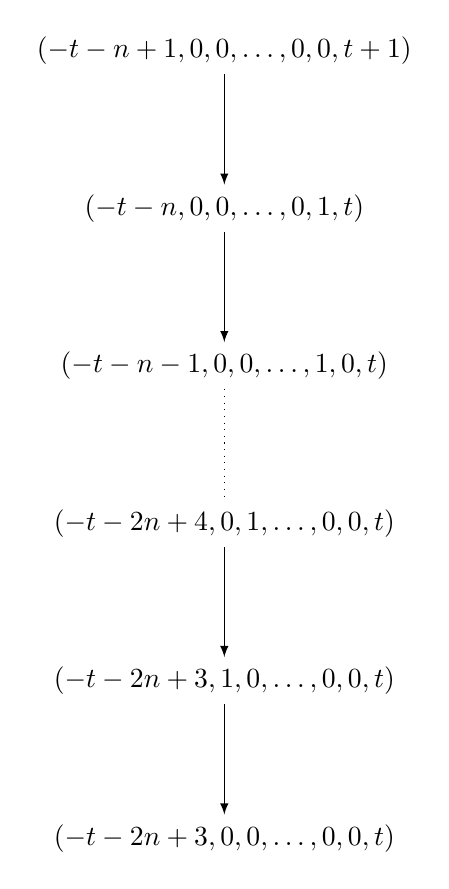
\begin{tikzpicture}[>=latex,line join=bevel,]

  \node (node_0) at (0,10) [draw,draw=none] {$\left(-t-n+1, 0, 0, \ldots, 0, 0, t+1\right)$};
  \node (node_1) at (0,8) [draw,draw=none] {$\left(-t-n, 0, 0, \ldots, 0, 1, t \right)$};
  \node (node_2) at (0,6) [draw,draw=none] {$\left(-t-n-1, 0, 0, \ldots, 1, 0, t \right)$};
  \node (node_3) at (0,4) [draw,draw=none] {$\left(-t-2n+4, 0, 1, \ldots, 0, 0, t \right)$};
  \node (node_4) at (0,2) [draw,draw=none] {$\left(-t-2n+3, 1, 0, \ldots, 0, 0, t \right)$};
  \node (node_5) at (0,0) [draw,draw=none] {$\left(-t-2n+3, 0, 0, \ldots, 0, 0, t \right)$};

  \draw [black,->] (node_0) edge (node_1);
  \draw [black,->] (node_1) edge (node_2);
  \draw [dotted] (node_2) to (node_3);
  \draw [black,->] (node_3) edge (node_4);
  \draw [black,->] (node_4) edge (node_5);
%
\end{tikzpicture}
\end{frame}

\begin{frame}{Example -- scalar products with positive roots}
$\mathrm{SO}^*(16)$: $\lambda = \left(a_{5} + 1\right)\omega_{5} + a_6\omega_6 + a_7\omega_7 - \left(2 \, a_{5} + 2 \, a_{6} + a_{7} + 8\right)\omega_{8}$
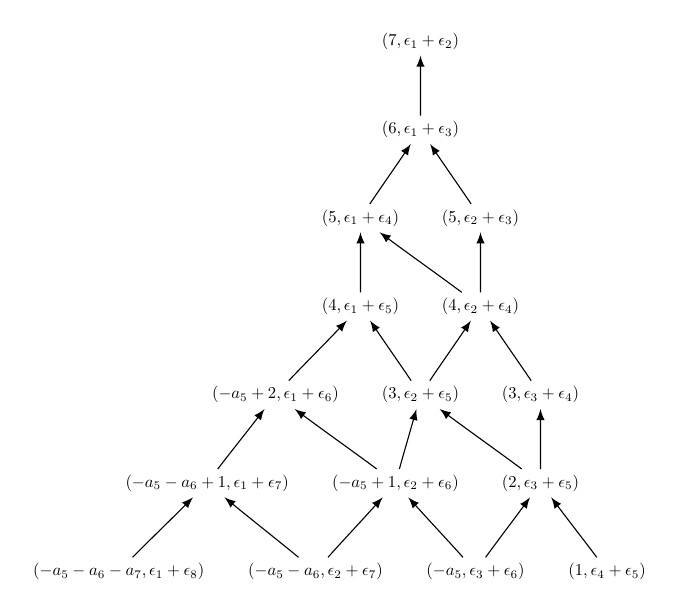
\begin{tikzpicture}[>=latex,line join=bevel,scale=0.6, every node/.style={transform shape}]
%%
\node (node_2) at (308.5bp,61.5bp) [draw,draw=none] {$(2, \epsilon_{3} + \epsilon_{5})$};
  \node (node_4) at (173.5bp,8.5bp) [draw,draw=none] {$(-a_{5} - a_{6}, \epsilon_{2} + \epsilon_{7})$};
  \node (node_3) at (269.5bp,8.5bp) [draw,draw=none] {$(-a_{5}, \epsilon_{3} + \epsilon_{6})$};
  \node (node_9) at (200.5bp,220.5bp) [draw,draw=none] {$(5, \epsilon_{1} + \epsilon_{4})$};
  \node (node_8) at (149.5bp,114.5bp) [draw,draw=none] {$(-a_{5} + 2, \epsilon_{1} + \epsilon_{6})$};
  \node (node_7) at (221.5bp,61.5bp) [draw,draw=none] {$(-a_{5} + 1, \epsilon_{2} + \epsilon_{6})$};
  \node (node_6) at (236.5bp,114.5bp) [draw,draw=none] {$(3, \epsilon_{2} + \epsilon_{5})$};
  \node (node_5) at (308.5bp,114.5bp) [draw,draw=none] {$(3, \epsilon_{3} + \epsilon_{4})$};
  \node (node_14) at (236.5bp,326.5bp) [draw,draw=none] {$(7, \epsilon_{1} + \epsilon_{2})$};
  \node (node_13) at (348.5bp,8.5bp) [draw,draw=none] {$(1, \epsilon_{4} + \epsilon_{5})$};
  \node (node_12) at (108.5bp,61.5bp) [draw,draw=none] {$(-a_{5} - a_{6} + 1, \epsilon_{1} + \epsilon_{7})$};
  \node (node_11) at (200.5bp,167.5bp) [draw,draw=none] {$(4, \epsilon_{1} + \epsilon_{5})$};
  \node (node_10) at (55.5bp,8.5bp) [draw,draw=none] {$(-a_{5} - a_{6} - a_{7}, \epsilon_{1} + \epsilon_{8})$};
  \node (node_1) at (272.5bp,167.5bp) [draw,draw=none] {$(4, \epsilon_{2} + \epsilon_{4})$};
  \node (node_0) at (272.5bp,220.5bp) [draw,draw=none] {$(5, \epsilon_{2} + \epsilon_{3})$};
  \node (node_15) at (236.5bp,273.5bp) [draw,draw=none] {$(6, \epsilon_{1} + \epsilon_{3})$};
  \draw [black,->] (node_12) ..controls (120.42bp,77.332bp) and (129.52bp,88.646bp)  .. (node_8);
  \draw [black,->] (node_8) ..controls (164.56bp,130.56bp) and (176.35bp,142.35bp)  .. (node_11);
  \draw [black,->] (node_10) ..controls (71.149bp,24.558bp) and (83.403bp,36.35bp)  .. (node_12);
  \draw [black,->] (node_6) ..controls (246.92bp,130.26bp) and (254.79bp,141.41bp)  .. (node_1);
  \draw [black,->] (node_1) ..controls (250.71bp,183.93bp) and (232.91bp,196.54bp)  .. (node_9);
  \draw [black,->] (node_3) ..controls (280.84bp,24.332bp) and (289.49bp,35.646bp)  .. (node_2);
  \draw [black,->] (node_4) ..controls (187.6bp,24.483bp) and (198.55bp,36.114bp)  .. (node_7);
  \draw [black,->] (node_9) ..controls (210.92bp,236.26bp) and (218.79bp,247.41bp)  .. (node_15);
  \draw [black,->] (node_0) ..controls (262.08bp,236.26bp) and (254.21bp,247.41bp)  .. (node_15);
  \draw [black,->] (node_11) ..controls (200.5bp,182.81bp) and (200.5bp,193.03bp)  .. (node_9);
  \draw [black,->] (node_7) ..controls (225.73bp,76.88bp) and (228.78bp,87.262bp)  .. (node_6);
  \draw [black,->] (node_13) ..controls (336.87bp,24.332bp) and (327.99bp,35.646bp)  .. (node_2);
  \draw [black,->] (node_15) ..controls (236.5bp,288.81bp) and (236.5bp,299.03bp)  .. (node_14);
  \draw [black,->] (node_5) ..controls (298.08bp,130.26bp) and (290.21bp,141.41bp)  .. (node_1);
  \draw [black,->] (node_1) ..controls (272.5bp,182.81bp) and (272.5bp,193.03bp)  .. (node_0);
  \draw [black,->] (node_7) ..controls (199.71bp,77.935bp) and (181.91bp,90.539bp)  .. (node_8);
  \draw [black,->] (node_2) ..controls (286.71bp,77.935bp) and (268.91bp,90.539bp)  .. (node_6);
  \draw [black,->] (node_6) ..controls (226.08bp,130.26bp) and (218.21bp,141.41bp)  .. (node_11);
  \draw [black,->] (node_3) ..controls (255.4bp,24.483bp) and (244.45bp,36.114bp)  .. (node_7);
  \draw [black,->] (node_2) ..controls (308.5bp,76.805bp) and (308.5bp,87.034bp)  .. (node_5);
  \draw [black,->] (node_4) ..controls (154.02bp,24.784bp) and (138.37bp,37.061bp)  .. (node_12);
%
\end{tikzpicture}
\end{frame}

\begin{frame}{$\lambda = -(t+n-1)\omega_1  + (t+1)\omega_{n-1}$}
$t=0$ -- Dirac, singularni, tabulka
	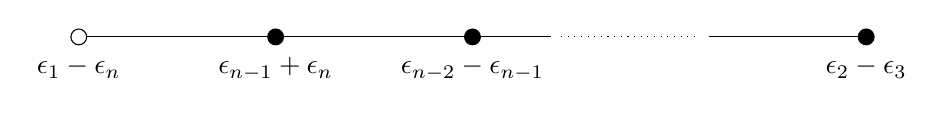
\begin{tikzpicture}
\draw (0 cm,0) -- (6 cm,0);
\draw (8 cm,0) -- (10 cm,0);
\draw[fill=white] (0 cm, 0 cm) circle (.1cm) node[below=4pt]{$\epsilon_{1} - \epsilon_{n}$};
\draw[fill=black] (2.5 cm, 0 cm) circle (.1cm) node[below=4pt]{$\epsilon_{n-1} + \epsilon_{n}$};
\draw[fill=black] (5 cm, 0 cm) circle (.1cm) node[below=4pt]{$\epsilon_{n-2} - \epsilon_{n-1}$};
\node (node_a) at (6 cm, 0 cm) {};
\node (node_b) at (8 cm, 0 cm) {};
\draw[fill=black] (10 cm, 0 cm) circle (.1cm) node[below=4pt]{$\epsilon_{2} - \epsilon_{3}$};
\draw [dotted] (node_a) to (node_b);
\end{tikzpicture}  
  {The reduced Hermitian symmetric pair for $\lambda = -(n-1)\omega_1  + \omega_{n-1}$}

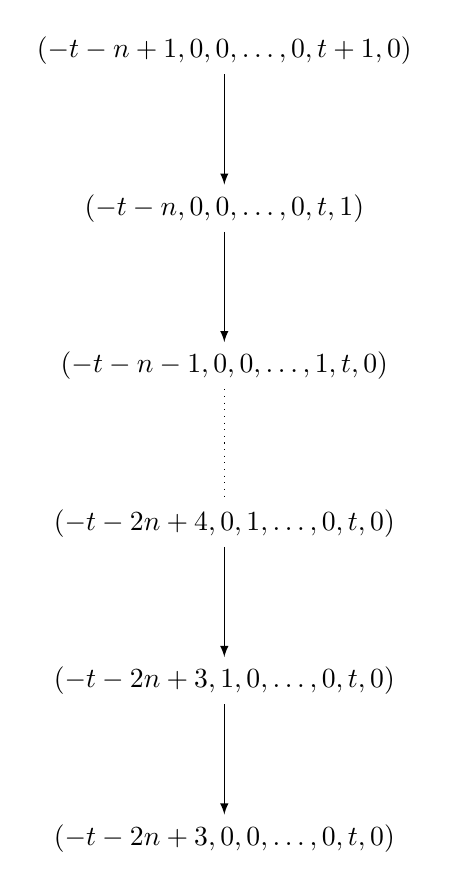
\begin{tikzpicture}[>=latex,line join=bevel,]

  \node (node_0) at (0,10) [draw,draw=none] {$\left(-t-n+1, 0, 0, \ldots, 0, t+1, 0\right)$};
  \node (node_1) at (0,8) [draw,draw=none] {$\left(-t-n, 0, 0, \ldots,  0, t, 1 \right)$};
  \node (node_2) at (0,6) [draw,draw=none] {$\left(-t-n-1, 0, 0, \ldots, 1,  t, 0 \right)$};
  \node (node_3) at (0,4) [draw,draw=none] {$\left(-t-2n+4, 0, 1, \ldots, 0,  t, 0 \right)$};
  \node (node_4) at (0,2) [draw,draw=none] {$\left(-t-2n+3, 1, 0, \ldots, 0,  t, 0 \right)$};
  \node (node_5) at (0,0) [draw,draw=none] {$\left(-t-2n+3, 0, 0, \ldots, 0,  t, 0 \right)$};

  \draw [black,->] (node_0) edge (node_1);
  \draw [black,->] (node_1) edge (node_2);
  \draw [dotted] (node_2) to (node_3);
  \draw [black,->] (node_3) edge (node_4);
  \draw [black,->] (node_4) edge (node_5);
%
\end{tikzpicture}
\end{frame}

\section{Conclusion}


\begin{frame}{Summary}

\begin{itemize}
 \item uniform and elementary construction of octonionic planes 
 \item generalization of Calderbank--Diemer construction to unitarizable highest weight modules
 \item software for nilpotent cohomology calculations 
 \item complete nilpotent cohomology of unitarizable highest weight modules in conformal case / partial results elsewhere
\end{itemize}

\end{frame}


{\setbeamercolor{palette primary}{fg=black, bg=white}

\begin{frame}[standout]

Thank you for your attention!

\end{frame}

}


\appendix


\begin{frame}[allowframebreaks]{References}


% \bibliography{../thesis}

% \bibliographystyle{abbrv}

\printbibliography


\end{frame}



\end{document}